%%%%%%%%%%%%%%%%%%%%%%%%%%%%%%%%%%%%%%%%%%%%%%%%%%%%%%%%%%%%
%%  This Beamer template was created by Cameron Bracken.
%%  Anyone can freely use or modify it for any purpose
%%  without attribution.
%%
%%  Last Modified: January 9, 2009
%%

\documentclass[xcolor=x11names,compress]{beamer}

%% General document %%%%%%%%%%%%%%%%%%%%%%%%%%%%%%%%%%
\usepackage{graphicx}
\usepackage{epstopdf}
\usepackage{tikz}
\usetikzlibrary{decorations.fractals}
\usepackage{animate}
%%%%%%%%%%%%%%%%%%%%%%%%%%%%%%%%%%%%%%%%%%%%%%%%%%%%%%


%% Beamer Layout %%%%%%%%%%%%%%%%%%%%%%%%%%%%%%%%%%
\useoutertheme[subsection=false,shadow]{miniframes}
\useinnertheme{default}
\usefonttheme{serif}
\usepackage{palatino}

\setbeamerfont{title like}{shape=\scshape}
\setbeamerfont{frametitle}{shape=\scshape}

\setbeamercolor*{lower separation line head}{bg=DeepSkyBlue4} 
\setbeamercolor*{normal text}{fg=black,bg=white} 
\setbeamercolor*{alerted text}{fg=red} 
\setbeamercolor*{example text}{fg=black} 
\setbeamercolor*{structure}{fg=black} 
 
\setbeamercolor*{palette tertiary}{fg=black,bg=black!10} 
\setbeamercolor*{palette quaternary}{fg=black,bg=black!10} 

\renewcommand{\(}{\begin{columns}}
\renewcommand{\)}{\end{columns}}
\newcommand{\<}[1]{\begin{column}{#1}}
\renewcommand{\>}{\end{column}}
%%%%%%%%%%%%%%%%%%%%%%%%%%%%%%%%%%%%%%%%%%%%%%%%%%




\begin{document}


%%%%%%%%%%%%%%%%%%%%%%%%%%%%%%%%%%%%%%%%%%%%%%%%%%%%%%
%%%%%%%%%%%%%%%%%%%%%%%%%%%%%%%%%%%%%%%%%%%%%%%%%%%%%%
\section{}
\begin{frame}
\title{Interdependent Evolution of Non-Spectral
Opinions and Social Networks}

\author{
	Fabian Russmann and Stefan Rustler\\
	{\it "Social State Physicists"}\\
}
\date{
	
	\vspace{1cm}
	Zurich, December 18 2012
}
\titlepage
\end{frame}

%%%%%%%%%%%%%%%%%%%%%%%%%%%%%%%%%%%%%%%%%%%%%%%%%%%%%%
%%%%%%%%%%%%%%%%%%%%%%%%%%%%%%%%%%%%%%%%%%%%%%%%%%%%%%
\section{}
\begin{frame}{Overview}
\tableofcontents
\end{frame}

%%%%%%%%%%%%%%%%%%%%%%%%%%%%%%%%%%%%%%%%%%%%%%%%%%%%%%
%%%%%%%%%%%%%%%%%%%%%%%%%%%%%%%%%%%%%%%%%%%%%%%%%%%%%%
\section{\scshape Introduction}
\subsection{Background and Motivation}
\begin{frame}{Background and Motivation}
\begin{itemize}

\item Opinion Formation (e.g. voter models) is a common and very fundamental problem in the social sciences

\item Goal: Modelling the \emph{co}evolution of both opinions and the underlying social network

\item \textbf{Does our social network shape the opinion we hold or does our opinion determine who is part of our network?}
\item Preview: Analogies to statistical physics, e.g. \emph{phase transitions} can be identified


\vspace{0.2in}

\item "Opinion" must be mutually exclusive and "non-spectral", e.g. brand preference, religious views...

\end{itemize}
\end{frame}

%%%%%%%%%%%%%%%%%%%%%%%%%%%%%%%%%%%%%%%%%%%%%%%%%%%%%%
%%%%%%%%%%%%%%%%%%%%%%%%%%%%%%%%%%%%%%%%%%%%%%%%%%%%%%
\section{\scshape The Model}

\subsection{Initial Setup}
\begin{frame}{Initial Setup}
\begin{itemize}
\item Random graph with $N$ nodes (opinion holder) and $M$ edges (social connection)
%self-edges and multi-edges not allowed!
\item Random opinion $g_i \in G$ assigned to node $i$ 
%different opinions denoted by a set of subsequent integers given by $G$. BUT NO CONTINUUM! EACH OPINION EQUALLY LIKELY: no pair exists whose opinions are more similar than another pair.
\item Nodes exchange information (opinion) via undirected edges
\item Externally set parameters:
\begin{itemize}
\item $N$ - number of nodes
\item $\gamma = \frac{N}{G}$ - average number of nodes per opinion
\item $k_{avg}=\frac{2M}{N}$ - average degree
\item $\Phi$ - reconnection probability
\end{itemize}
\end{itemize}
\end{frame}

%%%%%%%%%%%%%%%%%%%%%%%%%%%%%%%%%%%%%%%%%%%%%%%%%%%%%%

\subsection{Time Evolution Algorithm}
\begin{frame}{Time Evolution Algorithm}
\begin{enumerate}
\item Pick a random node $i$ with opinion $g_i$.  
\item (\textbf{a}) With probability $\Phi$ select at random one of the nodes $j$ that $i$ is connected to.
\begin{itemize}
\item If $g_i = g_j$, start over at step 1.
\item Otherwise, reconnect to a randomly chosen $j'$ of same opinion, i.e. $g_{j'} = g_i$.
\end{itemize}
\item (\textbf{b}) Otherwise, with probability $1-\Phi$ randomly select one of the neighboring vertices $j$ and change $g_i$ to $g_j$.
\item Repeat until \emph{consensus state} is achieved.
\end{enumerate}
\begin{center}
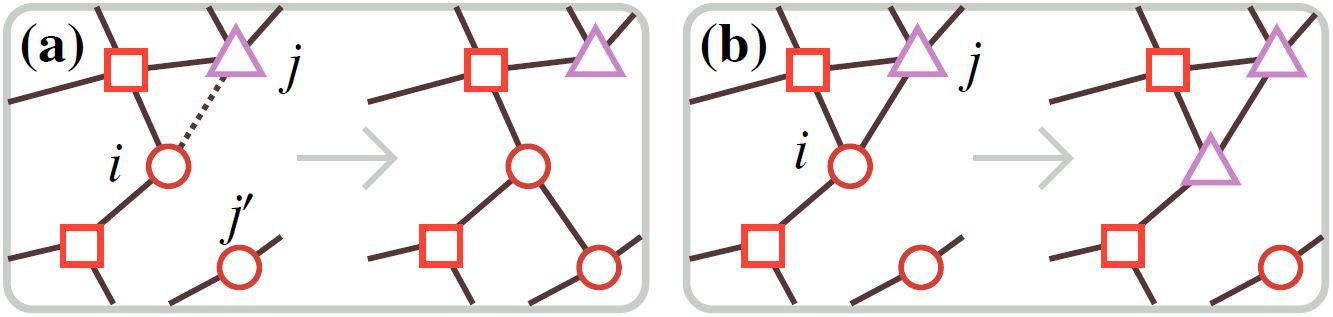
\includegraphics[scale=0.25]{Graphics/ModelIllustration.jpg}
\end{center}

\begin{tiny}
Figure: Holme and Newman, 2006 \cite{main paper}
\end{tiny}

\end{frame}

%%%%%%%%%%%%%%%%%%%%%%%%%%%%%%%%%%%%%%%%%%%%%%%%%%%%%%
%%%%%%%%%%%%%%%%%%%%%%%%%%%%%%%%%%%%%%%%%%%%%%%%%%%%%%
\section{\scshape Results}

\subsection{Cluster Size Distribution}
%Effect of different reconnection probabilities on different consensus states. Outline two intuitive, extreme scenarious first! Then quantitative treatment.
%Explain static picture first: 
	%Consensus state of particular PHI (N=..., Runs=200)
	%Normalized histogramm of cluster size s => P(s) (s€[1,N])
	%Explain first extreme scenario in detail (powlaw, gap, giantclust, 	     order phase)
%Explain last static picture:
	%Biggest cluster only 10%, smax=gamma, integer/zerobound=>Poisson
\begin{frame}{Cluster Size Distribution}
\animategraphics[scale=0.5]{9}{Graphics/ClustersizeDistr/}{10}{54}
\end{frame}

%%%%%%%%%%%%%%%%%%%%%%%%%%%%%%%%%%%%%%%%%%%%%%%%%%%%%%

\begin{frame}{Continuous Phase Transition?}
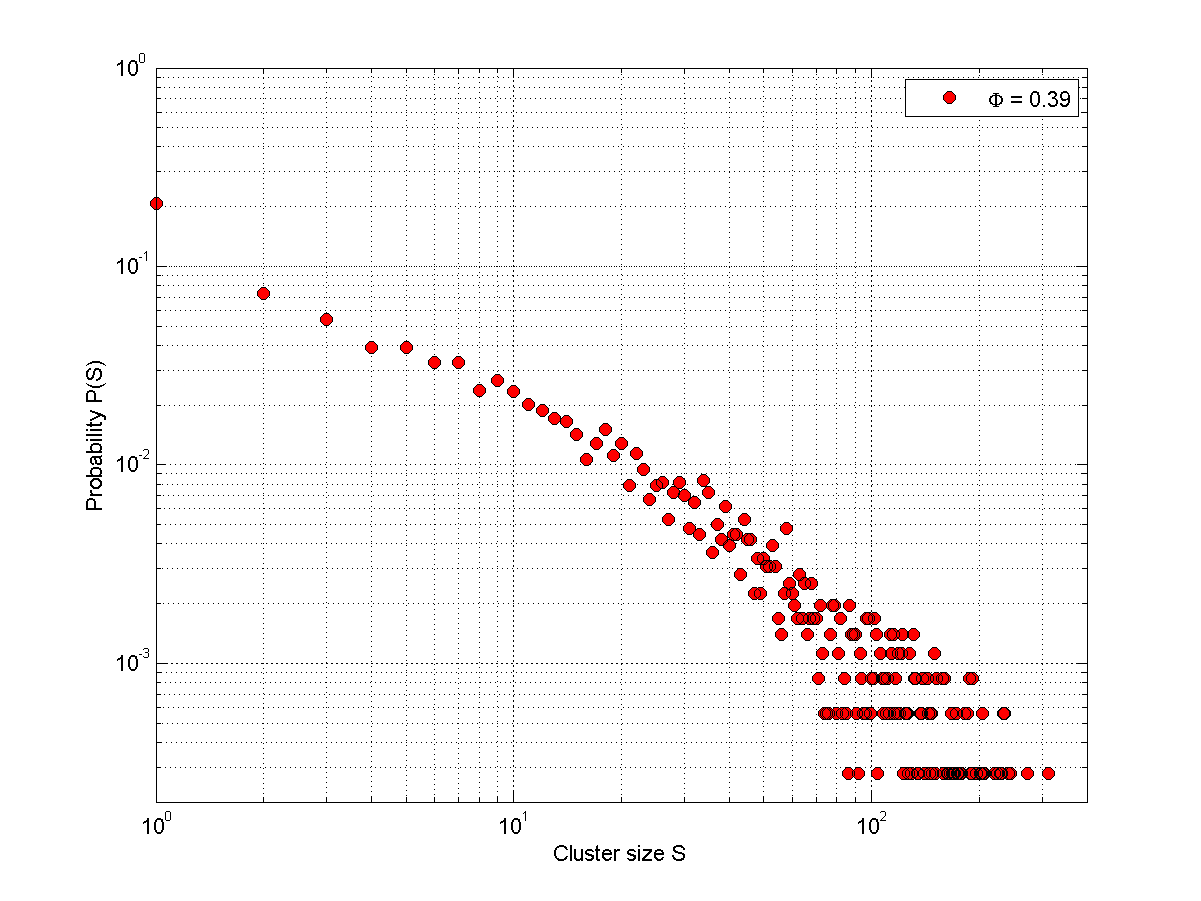
\includegraphics[scale=0.5]{Graphics/ClustersizeDistr/31.png}
\end{frame}

%%%%%%%%%%%%%%%%%%%%%%%%%%%%%%%%%%%%%%%%%%%%%%%%%%%%%%

\begin{frame}{Cluster Size Distribution}
\begin{itemize}
\item Ordered phase
\begin{itemize}
\item Low $\Phi$, i.e. tendency to change opinion
\item Small clusters follow power law distribution
\item Existence of giant cluster
\end{itemize}
\item Unordered phase
\begin{itemize}
\item High $\Phi$, i.e. tendency to keep opinion
\item Clusters follow Poisson-like distribution
\item No giant cluster!
\end{itemize}
\item Phase transition
\begin{itemize}
\item First guess: $\Phi_c = 0.39 \pm 0.05$
\item Power law behavior over the whole $s$-range
\item Order parameter $S=\frac{s_{max}}{N}$
\end{itemize}
\end{itemize}
\end{frame}

%%%%%%%%%%%%%%%%%%%%%%%%%%%%%%%%%%%%%%%%%%%%%%%%%%%%%%

\subsection{Phase Transition and Critical Point}

\begin{frame}{Phase Transition \& Critical Point}

\begin{center}
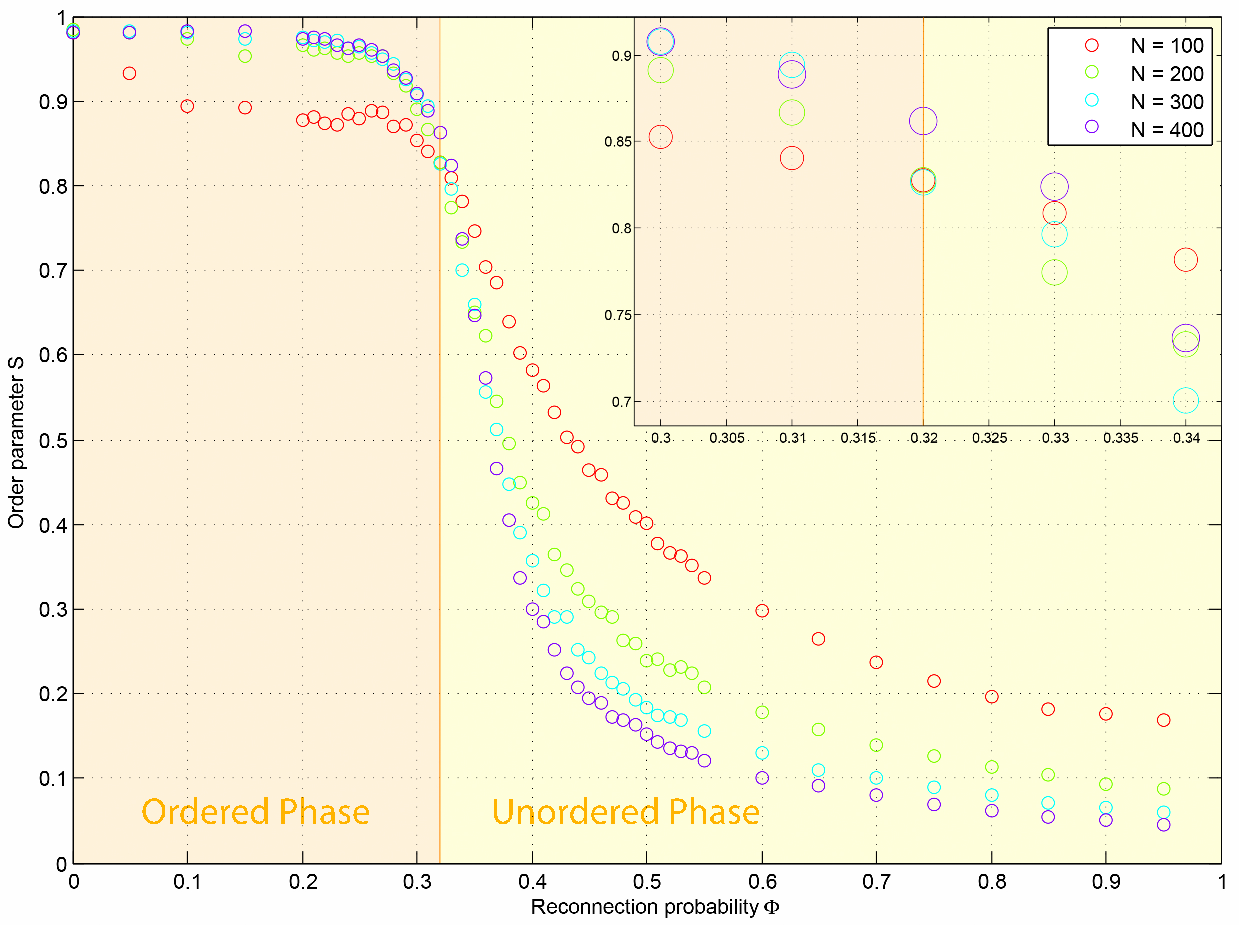
\includegraphics[scale=0.35]{Graphics/SvsPHI_combined.pdf}
\end{center}

\begin{itemize}
\item Really continuous phase transition
\item Bigger $N \rightarrow$ more dramatic transition
%Trend: steeper slope (more dramatic) for systems closer N-->inf (td limit)
\item $\Phi_c = 0.32 \pm 0.02$ independent of system size $N$
\item Weak agreement with $\Phi_c = 0.39 \pm 0.05$
\end{itemize}

\end{frame}



%%%%%%%%%%%%%%%%%%%%%%%%%%%%%%%%%%%%%%%%%%%%%%%%%%%%%%

\subsection{Convergence Time}
\begin{frame}{Convergence Time}

\begin{itemize}
\item Iterations per node to reach consensus as function of $\Phi$:
\item "Divergence" at some $\Phi_c$ for different $N$
\item Similar to divergent response functions in physics
\item Supporting phase transition interpretation, but difficult to find direct analogy to $\tau_{avg}$
\end{itemize}

\begin{figure}
    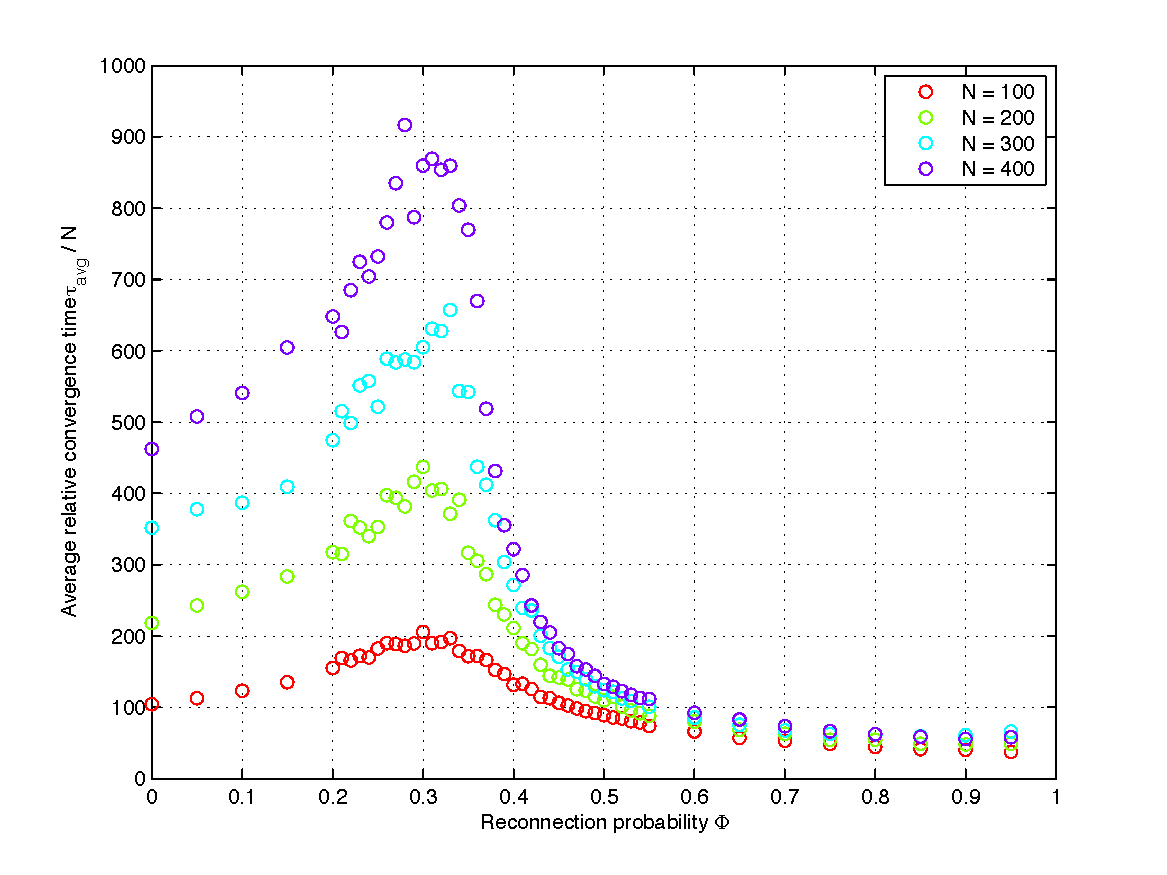
\includegraphics[scale=0.37]{Graphics/tau.pdf}
\end{figure}

\end{frame}

%%%%%%%%%%%%%%%%%%%%%%%%%%%%%%%%%%%%%%%%%%%%%%%%%%%%%%

\subsection{Comparisons to Empirical Data}
\begin{frame}{Comparisons to Empirical Data}

\begin{itemize}

\item Idea: Compare distributions of some "opinion" in real world to the model $\rightarrow$ identify and interpret corresponding $\Phi$

\vspace{0.1in}

\item \textbf{Religion:}
\item Worldwide distribution of religions follows power law: Neither adaptation nor reconnection dominate in the formation?




\begin{figure}
    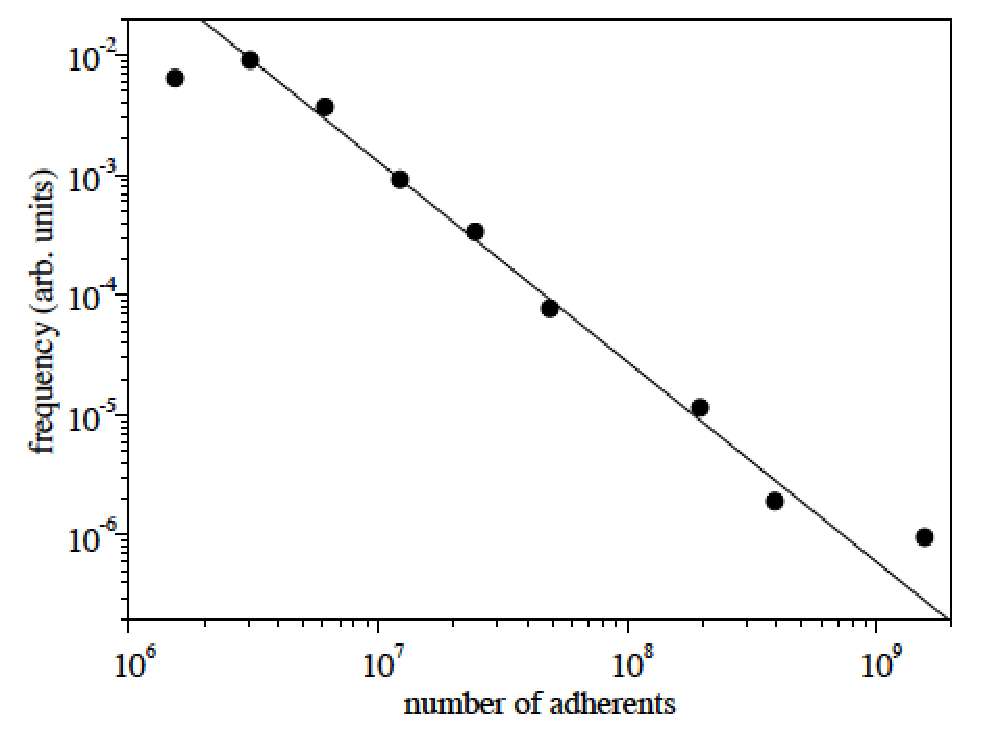
\includegraphics[scale=0.25]{Graphics/religion_power_law.pdf}
\end{figure}

\item Interpret $\Phi$ as an "intolerance indicator"?

\end{itemize}

\begin{tiny}
Zanette and Manrubia, 2000 \cite{religion power law}
\end{tiny}

\end{frame}

%%%%%%%%%%%%%%%%%%%%%%%%%%%%%%%%%%%%%%%%%%%%%%%%%%%%%%

\begin{frame}{Comparisons to Empirical Data}

\begin{itemize}


\item \textbf{Mobile Web Browsers:}
\item An example for opinion = brand preference
\item Contrast between giant cluster and "softer" distribution
\item Note: Plot is not a cluster size histogram!



\begin{figure}
    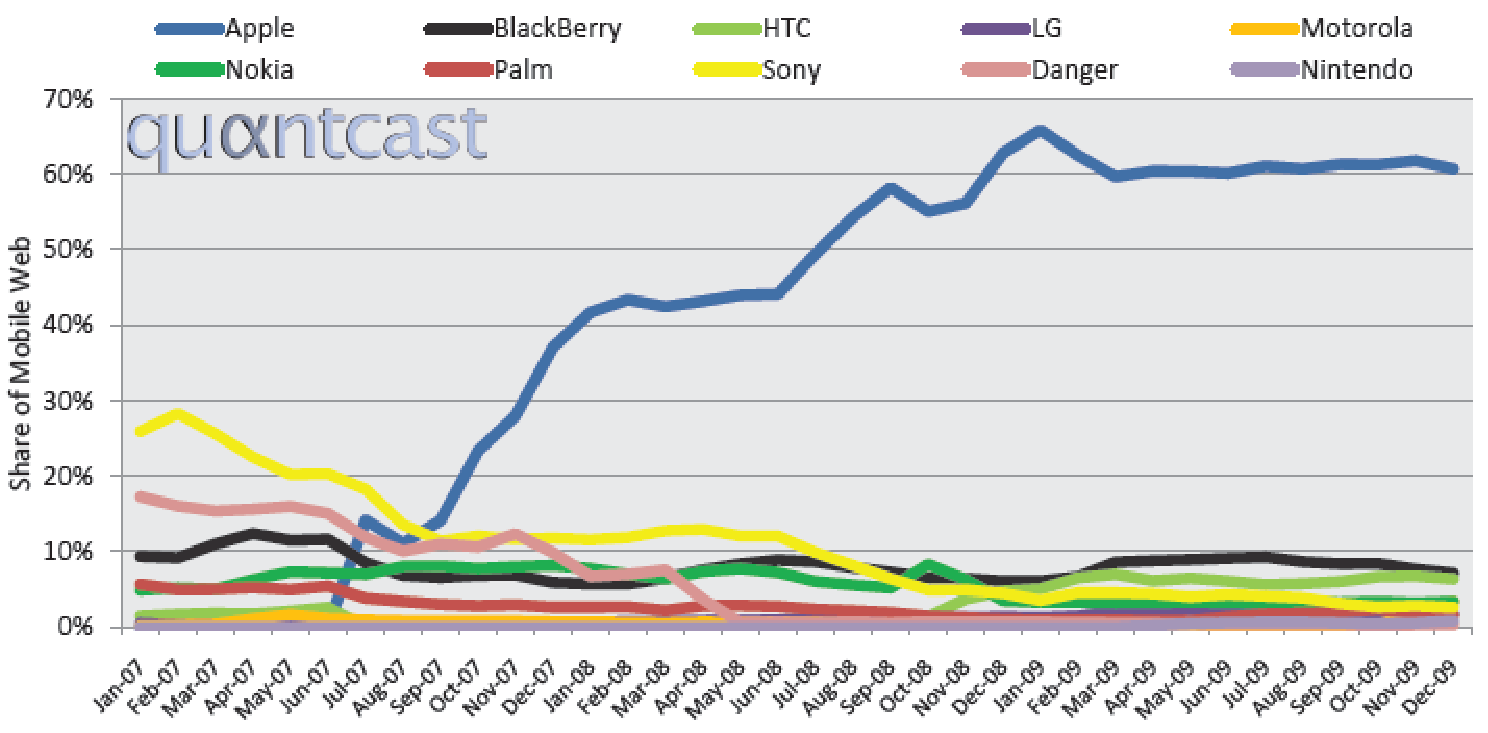
\includegraphics[scale=0.3]{Graphics/mobile_web.pdf}
\end{figure}

\item Interpret $\Phi$ as a "brand loyalty indicator"?

\end{itemize}

\begin{tiny}
Quantcast Review, 2009 \cite{quantcast}
\end{tiny}

\end{frame}



%%%%%%%%%%%%%%%%%%%%%%%%%%%%%%%%%%%%%%%%%%%%%%%%%%%%%%
%%%%%%%%%%%%%%%%%%%%%%%%%%%%%%%%%%%%%%%%%%%%%%%%%%%%%%
\section{\scshape Conclusion}

\subsection{Summary}

\begin{frame}{Summary}

\begin{itemize}
\item Interdependent evolution of opinions and networks, combining two mechanisms of adaption and reconnection determined by $\Phi$
\item Holme's and Newman's \cite{main paper} work could be reproduced with more realistic assumptions %No self- and multi-edges. No affecting of local consensus states.
\item Continuous phase transition
\begin{itemize}
\item $N$-independent critical value $\Phi_c = 0.32 \pm 0.02$
\item Divergent consensus time at $\Phi_c$
\end{itemize}
\end{itemize}

\textbf{Outlook}
\begin{itemize}
\item Variation of $\gamma$ (diversity) and $k_{avg}$ (density)
%Main paper suggests k-dep but gamma-indep of Phi_c.
\item Include analogue of "magnetic field" in model: "$informed$ $ agents$"?
%Phase diagrams, better check of analogies
\item Make opinions $spectral$
\item More detailed comparisons to empirical data
\end{itemize}

\end{frame}

%%%%%%%%%%%%%%%%%%%%%%%%%%%%%%%%%%%%%%%%%%%%%%%%%%%%%%

\subsection{References}
\begin{frame}{References}

\begin{tiny}


\begin{thebibliography}{9}

\bibitem{review}
R. Albert, A.-L. Barabasi. \emph{Statistical mechanics of complex
networks}. Rev. Mod. Phys, 74:47–98, 2002.

\bibitem{informed agents}
S. Brugger, C. Schwirzer. \emph{Opinion formation by "employed agents"
in social networks}. Project Report: Modelling and Simulating Social Systems with MATLAB, ETH Zurich, 2011.

\bibitem{voter model small world}
C. Castellano, D. Vilone, and A. Vespignani. \emph{Incomplete ordering
of the voter model on small-world networks}. Europhys.
Lett., 63:153–158, 2003.

\bibitem{erdos renyi}
P. Erd\H{o}s, A. R\'{e}nyi. \emph{On the evolution of random graphs}. Publications of the Mathematical Institute of the Hungarian Academy of Sciences 5: 17–61, 1960.

\bibitem{main paper}
P. Holme, M. E. J. Newman. \emph{Nonequilibrium phase transition in the coevolution of networks and opinions}. Physical Review E, vol. 74, Issue 5, id. 056108, 11/2006.

\bibitem{Nolting}
W. Nolting. \emph{Grundkurs Theoretische Physik 6: Statistische Physik}. Springer Berlin Heidelberg. 5. Aufl, 2004.

\bibitem{quantcast}
Quantcast, \emph{Quantcast Review of 2009 Mobile Web Trends}. "https://www.quantcast.com/inside-quantcast/2010/01/quantcast-review-of-2009-mobile-web-trends-mobile-web-share-up-110-in-north-america-and-148-globally" Accessed December 13, 2012.

\bibitem{voter model 2}
V. Sood, S. Redner. \emph{Voter model on heterogeneous graphs}. Phys. Rev. Lett., 94:178701, 2005.

\bibitem{religion power law}
D. H. Zanette,S. C. Manrubia. \emph{Vertical transmission of culture and the distribution of family names}. Physica A, 295:1–8, 2001.

\bibitem{ASSP}
A. Zheludev. \emph{Advanced solid state physics}. Lecture, ETH Zurich, Fall 2012.

\end{thebibliography}

\end{tiny}

\end{frame}

\end{document}
